\section{Discussion}
\label{sec:discussion}

\paragraph{Dictionary compression}
\sys includes infrastructure for per-size-class zstd dictionary
training.  We conducted six experiments varying CDict level,
dictionary capacity, sample count, and grouping strategy.
Dictionaries improve compression by up to 8\% at low zstd levels
(1--3), where the compressor's search window is too small to discover
cross-page patterns independently.  At level~9, the search window is
large enough that dictionaries provide no benefit beyond frame
overhead.  More importantly, CDict objects consume 430--686\,KiB
each, and training buffers add 256\,KiB per size class.  Even with
aggressive optimizations (CDict at level~3, 16\,KiB capacity,
maximum 8 trained classes), dictionaries reduce RSS savings by
8.9\pp on average (Figure~\ref{fig:dict_overhead}).  \sys preserves
the training infrastructure but disables it by default.

\begin{figure}[t]
\centering
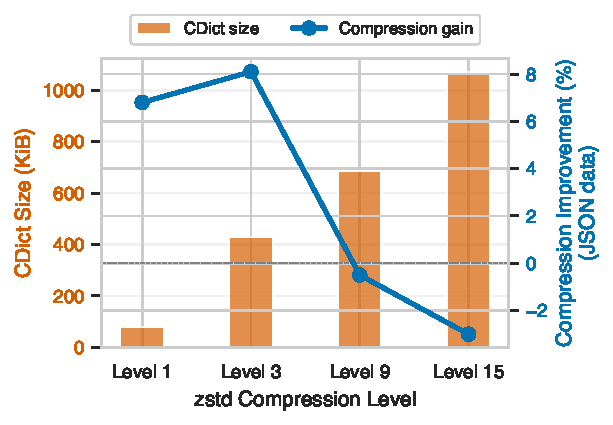
\includegraphics[width=\columnwidth]{figures/dict_overhead.pdf}
\caption{\textbf{Dictionaries add memory overhead without
  improving compression} (\S\ref{sec:discussion}).  CDict memory
  cost vs.\ compression benefit on JSON data.}
\label{fig:dict_overhead}
\end{figure}

\paragraph{Multi-page compression}  Compressing 2--4 contiguous
pages as a unit improves ratios by 2--4\pp (e.g., JSON-LZ4 from
30.2\% to 26.2\% with 4-page groups).  However, all pages in a
group must be simultaneously cold, and a fault on any page requires
decompressing the entire group.  Mixed hot/cold page groups prevent
compression entirely.  The 2--4\pp gain does not justify the added
complexity and worst-case decompression cost.

\punt{\paragraph{WKdm and modern page sizes}  The macOS VM compressor uses
WKdm, designed for 4\,KiB pages containing pointer-heavy C
structures.  On 16\,KiB pages with text or serialized data, WKdm
achieves 93--99\% ratios.  Even on binary data, LZ4 outperforms WKdm
(5.8\% vs.\ 15.6\% on SQLite pages).  This gap motivates
byte-oriented compressors for heap data.}

\paragraph{Design principles for compressible pages}
The allocator substrate comparison (\S\ref{sec:eval:allocator})
and pipeline decomposition (\S\ref{sec:eval:pipeline}) together
suggest a hierarchy of importance for compression-friendly allocator
design:

The dominant factor is \emph{having a compression pipeline at all}:
the compress-only variant achieves 32--61\% RSS reduction with an
unmodified system allocator, and no allocator design choice can
substitute for a pipeline that monitors access patterns, compresses
cold pages, and decompresses on demand.  Among page-content
optimizations, \emph{zero-on-free} contributes most, improving
compression ratios by 2--4\% for every allocator tested (DieHarder
zeros for security; \sys zeros for compression; the effect on page
content is the same).  \emph{External metadata}---storing freelists
and bitmaps outside data pages---has a modest effect ($\sim$2\%) and
is dominated by zeroing.  \emph{Arena segregation} helps on
heterogeneous workloads but provides little benefit
when data is already structurally uniform.  Finally,
\emph{allocation layout}---sequential vs.\ randomized---affects
compression more than metadata placement: system malloc's sequential
layout compresses better than DieHard's randomized layout despite
embedded freelists.  Mesh confirms this: it shares DieHard's
external bitmap metadata but uses a conventional layout, achieving
compressibility on par with system malloc (7.9\% vs.\ 7.4\%).

These findings generalize beyond \sys: any system that compresses
heap pages (including OS-level compressors) would benefit from
allocators that zero freed slots and produce sequential layouts.

\paragraph{Synergy between pipeline and allocator}
The compress-only experiment (\S\ref{sec:eval:pipeline}) shows
that \sys's compression pipeline achieves substantial benefit
even atop an allocator that was not designed for compression.  On
small-object workloads (SQLite), compress-only matches
or exceeds full \sys.  The allocator design contributes
substantially on large-object workloads (RocksDB: +25\pp)
where freelist pollution spans entire pages, and \sys's integrated
design avoids the hash-map-based page tracking overhead that costs
compress-only 7--18\% throughput.  The pipeline could also be
deployed as a standalone library,
though the integrated design avoids the overhead of external page
tracking and provides additional benefit for large allocations.

The multi-allocator comparison (\S\ref{sec:eval:apps})
reinforces this point: across seven alternative allocators
(mimalloc, jemalloc, tcmalloc, Hoard, Mesh, DieHard, DieHarder),
none reduces RSS below its fill level.  Mesh's virtual-memory
remapping helps on workloads with sparse pages (35\% on RocksDB,
42\% on DuckDB) but provides no benefit when pages are fully
occupied.  Without a compression
pipeline, an allocator can only return empty pages to the OS.

\paragraph{Limitations}  Decompression adds 1--10\,$\mu$s per
fault (Table~\ref{tab:apps}).  Workloads with uniform access
patterns across the entire heap (no cold pages) see no benefit.
The syscall interposition layer covers 20 functions; unusual
syscalls accessing heap buffers may require additional wrappers.
The bootstrap allocator's memory is never freed, contributing a
fixed overhead of $\sim$25\,MiB for page state arrays and
compression contexts.

\paragraph{Adaptive size classes}  \sys uses a conventional
36-class scheme designed to bound internal fragmentation.  An
alternative would split size classes further based on compression
feedback: if objects in the same class but from different call
sites compress differently, the allocator could create sub-classes
to increase page homogeneity.  Arena segregation already
approximates this by routing call sites to separate arenas,
creating $4 \times 36 = 144$ effective buckets.  Finer splitting
could help but increases the number of live spans and thus
external fragmentation; we leave this tradeoff to future work.

\paragraph{Security}  Zeroing freed objects prevents information
leakage through stale heap data, a concern first addressed by
Chow et al.'s \emph{secure deallocation}~\cite{chow2005shredding}.
\sys's zero-on-free provides a similar security benefit, though
its primary purpose is compression effectiveness.
